% !TEX root = ../main.tex
\lecture{3}{2026-09-28}{Woche 3}

\section{Erfolgsrechnung}
\begin{itemize}
    \item Im Vergleich zur Bilanz
        \subitem kann veränderung der Lage der Aktiven und Passiven abbilden (Wertschöpfungsabbildung)
        \subitem Nicht Periodenkummulativ (also kein Anfangsbestand)
    \item Erfolgsrechnung
    \begin{itemize}
            \item Abbildung der Ertragslage meistens während eine jährlichen Periode
            \item besteht aus 2 Kontoarten
            \item Verbuchung von \textbf{Aufwand} (\textit{Aktiven}) und \textbf{Ertrag} (Passiv) nach ähnlicher Logik wie Bilanzen
            \item keine Anfangsbestände weil formell noch keine Erträge oder Gewinne erzielt wurden zu Beginn einer Periode
    \end{itemize}
\end{itemize}
\subsection{Ertrag und Aufwand}
\textbf{Ertragskonten} halten folgendes fest: 
\begin{itemize}
    \item Soll oder Aufwand (-)
    \begin{itemize}
            \item $\downarrow$ Aktivkonten
            \item $\uparrow$ Passivkonten
        \item Saldo (Summe)
        
    \end{itemize}
    \item Haben oder Korrektur (+) \textit{nur bei Veränderung einer bereits eingetragenen Buchungstatsache}
    \begin{itemize}
        \item $\uparrow$ Aktivkonten
        \item $\downarrow$ Passivkonten
    \end{itemize}
\end{itemize}
\pagebreak
\textbf{Aufwandkonten} umgekehrt zum Ertragskonto (Prinzip der Doppelten Buchhaltung)
\begin{itemize}
    \item Soll oder Aufwand (+)     
          \begin{itemize}
            \item $\uparrow$  Aktivkonten
              \item $\downarrow$Passivkonten
          \end{itemize}
    \item Haben oder Korrekturen (-) \textit{nur bei Veränderung einer bereits eingetragenen Buchungstatsache}
          \begin{itemize}
            \item $\downarrow$ Aktivkonten
            \item $\uparrow$ Passivkonten 
             \item Saldo (Summe)
          \end{itemize}
\end{itemize}
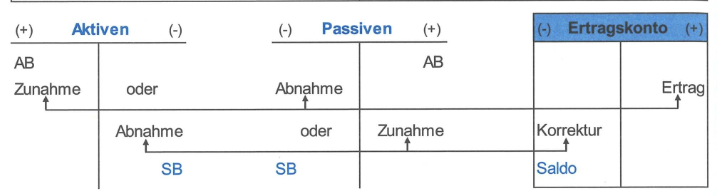
\includegraphics[width=\textwidth,height=0.7\textheight,keepaspectratio]{figures/Ertragskonto.png}

\subsubsection{Buchungsvorgang}
\begin{enumerate}
    \item Buchungstatsache feststellen
    \item 1x Tangierte Bilanzkonto
    \item 1x tangierte Erfolgskonto (Aufwand oder Ertrag)
    \item Bei Gewinn wird vom aktiven \textit{Soll} (+) ins \textit{Haben} vom Ertragskonto (+) 
    \item Bei Verlust wird vom aktiven \textit{Haben} (-) ins \textit{Soll} vom Aufwand (+) \footnote{Der Mehrwert, der hier keine Quelle hat oder aus dem Nichts geschöpft wird, wird somit aus der Differenz von Aufwand und Ertrag abgebildet, und Doppelte Buchhaltung bleibt bestehen, weil 1 Bilanzkonto an einem Erfolgskonto.}
    \item Bei Notwendigkeit von Korrektur einer Buchungstatsache, wird im Selben Erfolgskonto wieder abgezogen oder zugerechnet

\end{enumerate}
\subsection{Aufbau und Erfolgsursachen}
Die Erfolgskonten sind wesentlich für die Unternehmensbewertung. Sie zeigen qualitativ und quatitative Ursachen der Gewinne/Verluste.

\subsubsection{Gliederung Ursachen}
Nach Tätigkeit werden Erfolgskonten sortiert.
\begin{itemize}
    \item Betriebsbereich (primäre Aktivitätsertrage)
    \subitem zB Personalaufwand, Warenaufwand, Mietaufwand 
    \item Finanzbereich (Finanzierung)
    \subitem Zinsaufwände oder gutschriften, Dividendenzahlungen
    \item Neutralerbereich (weder noch)
    \begin{itemize}
        \item Periodenfremde Erträge, die in einer anderen Periode nicht gebucht wurden
        \item Ausserordentlichen Erträge
        \subitem Aufwendung aus Schadensfall, Schenkungen, Restrukturierung 
        \item Unternehmensfremd (aus sekundäre Tätigkeit) \footnote{nicht immer klar zu trennen}
        \subitem Immobilienaufwand- ertrag, wenn Real Estate keine Haupttätigkeit
    \end{itemize} 
\end{itemize}

\subsubsection{Problematik}
Mögliche Manipulationsfälle, worin Gewinne aus ausserordentlichen Erträge im primären Betriebsbereich gebucht wurden. So könnte die Unternehmenslage als stabil gefälscht werden. 

\subsubsection{Aufbau - Staffelform}

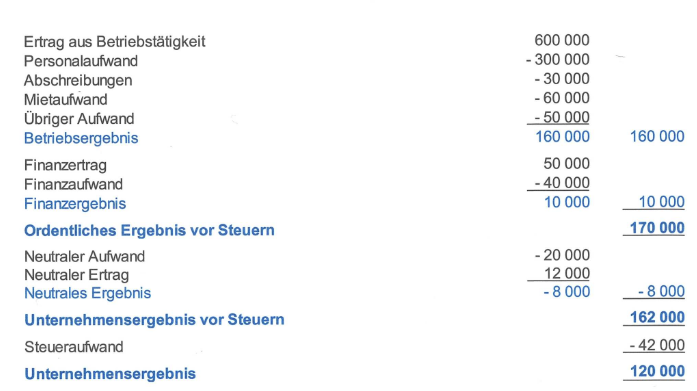
\includegraphics[width=\textwidth,height=0.7\textheight,keepaspectratio]{figures/Erfolgsrechnung_Aufbau.png}

\subsubsection{Aufbau - Kontoform}
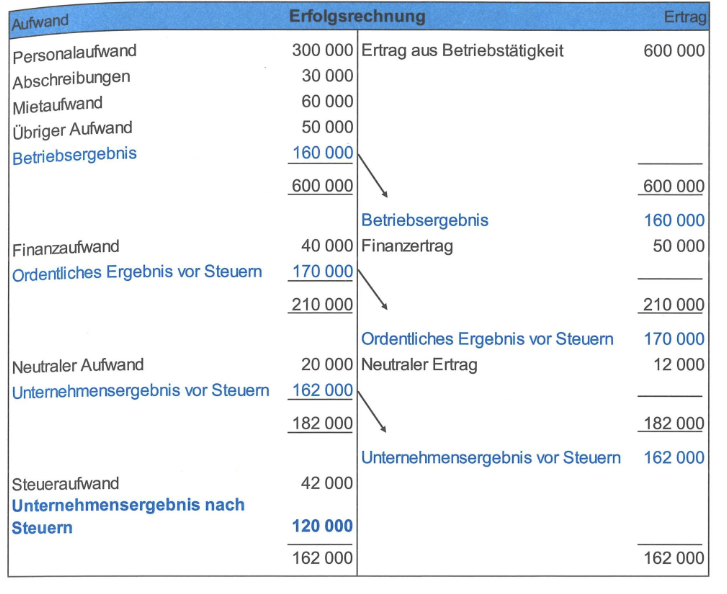
\includegraphics[width=\textwidth,height=0.7\textheight,keepaspectratio]{figures/Erfolgsrechnung_Kontoform.png}
